%%%% 補助スライド
\appendix
\backupbegin

\begin{frame}{}\Huge
 Appendix
\end{frame}

\begin{frame}{クイーングラフ}
 \begin{block}{クイーングラフ}
  $n\times n$のチェス盤について各マスを頂点とし,
  クイーンが移動できるマス同士が辺で結ばれているグラフを
  \structure{クイーングラフ}といい,$Q_n$と表す.
 \end{block}
 \begin{exampleblock}{クイーングラフの例: $Q_3$}
  例として,サイズ$3 \times 3$のチェス盤と
  クイーングラフ$Q_3$の対応関係を下図に示す.
  \begin{figure}[htb]
   \label{ex:queengraph_3}
   \begin{minipage}[b]{0.2\linewidth}
    \centering
    \begin{tikzpicture}
 \draw[gray] (-0.75,-0.75)--(-0.75,0.75);
 \draw[gray] (-0.25,-0.75)--(-0.25,0.75);
 \draw[gray] (0.25,-0.75)--(0.25,0.75);
 \draw[gray] (0.75,-0.75)--(0.75,0.75);
 \draw[gray] (-0.75,-0.75)--(0.75,-0.75);
 \draw[gray] (-0.75,-0.25)--(0.75,-0.25);
 \draw[gray] (-0.75,0.25)--(0.75,0.25);
 \draw[gray] (-0.75,0.75)--(0.75,0.75);
 \draw[red][<->] (0.5,-0.5)--(-0.5,0.5);
 \draw[red][<->] (-0.5,-0.5)--(0.5,0.5);
 \draw[red][<->] (0,-0.5)--(0,0.5);
 \draw[red][<->] (-0.5,0)--(0.5,0);
 \matrix[matrix of nodes,nodes={inner sep=10pt,text width=1cm,
align=center,minimum height=1cm}]{
  &  & \symqueen  \\
  &  & \\
  &  &  \\};
\end{tikzpicture}
   \end{minipage} 
   \begin{minipage}[b]{0.5\linewidth}
    \centering
    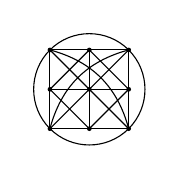
\begin{tikzpicture}
 \draw (-0.5,-0.5)--(-0.5,0.5);
 \draw (0,-0.5)--(0,0.5);
 \draw (0.5,-0.5)--(0.5,0.5);
 \draw (-0.5,-0.5)--(0.5,-0.5);
 \draw (-0.5,0)--(0.5,0);
 \draw (-0.5,0.5)--(0.5,0.5);
 \draw (-0.5,-0.5)--(0.5,0.5);
 \draw (-0.5,0.5)--(0.5,-0.5);
 \draw (-0.5,0)--(0,0.5);
 \draw (-0.5,0)--(0,-0.5);
 \draw (0.5,0)--(0,0.5);
 \draw (0.5,0)--(0,-0.5);
 \draw (-0.5,0.5) to [out=45,in=135] (0.5,0.5);
 \draw (0.5,0.5) to [out=315,in=45] (0.5,-0.5);
 \draw (0.5,-0.5) to [out=225,in=315] (-0.5,-0.5);
 \draw (-0.5,-0.5) to [out=135,in=225] (-0.5,0.5);
 \draw (-0.5,-0.5) to [out=75,in=195] (0.5,0.5);
 \draw (-0.5,0.5) to [out=345,in=105] (0.5,-0.5);
 \foreach \x in {-0.5,0,0.5}
  \foreach \y in {-0.5,0,0.5}
   \fill (\x,\y) circle (0.03);
\end{tikzpicture}
   \end{minipage}
  \end{figure}
 \end{exampleblock}
\end{frame}


%
%クイーン支配問題の支配数等に関する背景知識
%

\begin{frame}{クイーン支配問題の支配数}
  \begin{itemize}
    \item クイーン支配問題の支配数は,1862年に文献[Jaenisch,1862]で
	    $\gamma(Q_8)=5$が示されてから研究されている.
    \item $n=3,11$を除いた$n \leq 132$で $\lceil n/2 \rceil 
	    \leq \gamma(Q_{n}) \leq \lceil n/2 \rceil +1$
	 であることが証明されている[\"{O}sterg{\aa}rd,Weakley,2001].
%    \item THE ON-LINE ENCYCLOPEDIA OF INTEGER SEQUENCES には,
%    $1\leq n\leq 25$に対する$\gamma(Q_n)$
%    が掲載されている~\footnote{\url{https://oeis.org/A075458}}.
  \end{itemize}
 \begin{exampleblock}{$Q_{n}$の支配数$(1 \leq n \leq 20)$}
  \centering
  \begin{tabular}{c|c||c|c||c|c||c|c}%\hline
    $n$ & $\gamma(Q_{n})$ & $n$ & $\gamma(Q_{n})$ &$n$ & $\gamma(Q_{n})$ &$n$ & $\gamma(Q_{n})$ \\ \hline
    1 &1 &6 &3 &11 &5 &16 &9 \\ %\hline
    2 &1 &7 &4 &12 &6 &17 &9 \\ %\hline
    3 &1 &8 &5 &13 &7 &18 &9 \\ %\hline
    4 &2 &9 &5 &14 &8 &19 &10 \\ %\hline
    5 &3 &10 &5 &15 &9 &20 &11 \\ %\hline
  \end{tabular}
 \end{exampleblock}
\end{frame}


\begin{frame}{基本符号化の制約モデル}
 \begin{block}{}
  \begin{description}
   \item[{\color{black} (アトム$q_{ij}$})] 
	      $q_{ij} \in \{0,1\} 
	      \qquad (1 \leq i,j \leq n)$ \par
	      \begin{itemize}
	       \item $q_{ij}$が1のとき,マス$(i,j)$にクイーンが
		     配置されることを意味する.
	      \end{itemize}
   \item[{\color{black}(制約 1)}] 
	      $\sum\limits_{i,j=1}^{n} q_{ij} = k$ \par
	      \begin{itemize}
	       \item $n \times n$上のクイーンの総数が
		     $k$個であることを意味する.
	      \end{itemize}
   \item[{\color{black}(制約 2)}] 
	      $\bigvee\limits_{i',j' \in A_{ij}}q_{i'j'} > 0$ \par
	      \begin{itemize}
	       \item マス$(i,j)$に移動できるクイーンが一つ以上
		     配置されていることを意味する.
	      \end{itemize}
	      
  \end{description}
 \end{block}
 \begin{alertblock}{}
  \begin{itemize}
   \item (制約 2)中に同じ部分式が何度も出現してしまう(以下は$Q_3$の例).
   \begin{align*}
    {\color{red} q_{11}>0 \vee q_{12}>0 \vee q_{13}>0} 
    \vee q_{21}>0 \vee q_{22}>0 \vee q_{31}>0 \vee q_{33}>0 \\
    {\color{red} q_{11}>0 \vee q_{12}>0 \vee q_{13}>0} 
    \vee q_{21}>0 \vee q_{22}>0 \vee q_{23}>0 \vee q_{32}>0 \\
    {\color{red} q_{11}>0 \vee q_{12}>0 \vee q_{13}>0} 
    \vee q_{22}>0 \vee q_{23}>0 \vee q_{31}>0 \vee q_{33}>0 
   \end{align*}
  \end{itemize}
 \end{alertblock}
\end{frame}

\begin{frame}{改良符号化の制約モデル}
 \begin{alertblock}{}
  改良符号化では,基本符号化において複数回出現する,\\
  リテラルの選言部分をまとめるための補助アトムを導入する.
 \end{alertblock}
 \begin{block}{}
  \begin{itemize}
   \item 各行$i$に対してアトム$r_{i}$と制約3を追加する.
	 \begin{description}
	  \item[{\color{black} (アトム$r_{i}$})] 
		     $r_{i} \in \{0,1\}$  $(1 \leq i \leq n)$ 
		     \vskip .5em
	  \item[{\color{black} (制約 3)}] 
		     $r_{i}>0 \rightarrow \bigvee\limits_{i',j' 
		     \in R_{ij}}q_{i'j'} = 1 \quad (1\leq i \leq n)$ \par
		     $r_{i}$が1のとき,行$i$にクイーンがひとつ以上
		     配置されることを意味する.
	 \end{description}
   \item 各列,各右上がり対角線,各右下がり対角線に対しても同様に\\
	 補助アトム$c_j$,$u_{i+j}$,$d_{i-j}$と(制約 4),
	 (制約 5),(制約 6)を追加する
  \end{itemize} 
 \end{block}
 \begin{block}{}
  \begin{itemize}
   \item 基本符号化の(制約 2)を削除し,(制約 7)を追加する.
	 \begin{description}
	  \item[{\color{black} (制約 7)}] $r_{i} \vee c_{j} \vee u_{i+j} 
		     \vee d_{i-j} > 0  \qquad 1\leq i,j \leq n$ 
	 \end{description}
  \end{itemize} 
 \end{block}
\end{frame}

\begin{frame}{部分和符号化の制約モデル}
 \begin{alertblock}{}
  部分和符号化では,各行,各列,各対角線ごとのクイーンの個数を表す
  補助アトムを導入し,行方向,列方向,対角線方向それぞれに対し
  クイーンの総数に関する(制約 8)を追加する.
 \end{alertblock}
 \begin{block}{}
  \begin{description}
   \item[{\color{black} (アトム$r_{i}$)}] $r_{i} \in \{0,...,k\} \qquad (1 \leq i \leq n)$
   \item[{\color{black} (制約 8)}] $\sum\limits_{i=1}^{n}r_{i} = \sum\limits_{j=1}^{n}c_{j} = \sum\limits_{i+j=2}^{2n}u_{i+j} = \sum\limits_{i-j=1-n}^{n-1}d_{i-j} = k$
  \end{description}
各列,各右上がり対角線,各右下がり対角線に対しても同様に\\
補助アトム$c_j$,$u_{i+j}$,$d_{i-j}$と(制約 9),(制約 10),(制約 11)を追加する.
 \end{block}
\end{frame}

\begin{frame}\frametitle{部分和符号化における行方向の追加制約による推論}
 \begin{block}{}
  \begin{description}
   \item[(追加制約1)] $r_{i}=\sum\limits_{(i',j')\in \mbox{行}i} 
	      q_{i'j'} \qquad (1 \leq i \leq n)$ 
	      \begin{itemize}
	       \item 行$i$のクイーンの個数を$r_i$とする.
	      \end{itemize}
   \item[(追加制約2)] $\sum\limits_{i=1}^{n}r_{i} = k$
	      \begin{itemize}
	       \item 行ごとのクイーンの合計は盤面全体の数に一致する.
	      \end{itemize}
  \end{description}
 \end{block}
 \begin{exampleblock}{例:$n=5,k=3$のとき}
  \begin{columns}
   \begin{column}{0.30\textwidth}
    \centering
    %%%%%%%%%%%%%%%%%%%%%%%%%%%%%%%%%%%%%%%%%%%%%%%%%%
% 実行例(t=0) (第6章で使う)
%%%%%%%%%%%%%%%%%%%%%%%%%%%%%%%%%%%%%%%%%%%%%%%%%%

\begin{tikzpicture}[scale=0.6]

  % 設定
  \tikzset{node/.style={circle,draw=black}}
 
  \definecolor{col_r}{RGB}{230,0,18}
  %\definecolor{col_b}{RGB}{0,104,183}
  \definecolor{col_b}{RGB}{51,51,179}
  \definecolor{col_y}{RGB}{255,251,0}
  \definecolor{col_g}{RGB}{0,96,0}
 
  % 補助線
  % \draw [help lines,blue] (0,0) grid (20,6);
 
  % node %
  \node[node, fill=col_y!70] (node1){\textbf{1}};
  \node[node, fill=col_b!70, right=of node1] (node2){\textbf{2}};
  \node[node, fill=col_y!70, below=of node1] (node3){\textbf{3}};
  \node[node, fill=col_g!70, below=of node2] (node4){\textbf{4}};
 
  \foreach \u / \v in {node1/node2, node2/node3, node2/node4, node3/node4}
  \draw (\u) -- (\v);
 \end{tikzpicture}
 
 %%%%%%%%%%%%%%%%%%%%%%%%%%%%%%%%%%%%%%%%%%%%%%%%%%%%%%%%%%
 %%% Local Variables:
 %%% mode: japanese-latex
 %%% TeX-master: paper.tex
 %%% End:
 
   \end{column}
   \begin{column}{0.30\textwidth}
    \centering
    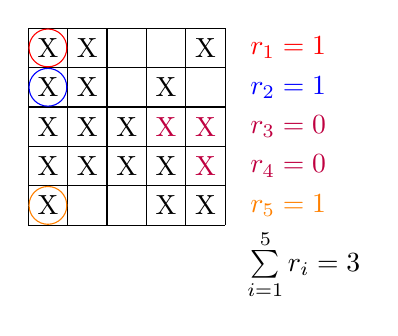
\begin{tikzpicture}
 \draw (0,0)--(2.5,0);
 \draw (0,0.5)--(2.5,0.5);
 \draw (0,1.0)--(2.5,1.0);
 \draw (0,1.5)--(2.5,1.5);
 \draw (0,2.0)--(2.5,2.0);
 \draw (0,2.5)--(2.5,2.5);
 \draw (0,0)--(0,2.5);
 \draw (0.5,0)--(0.5,2.5);
 \draw (1.0,0)--(1.0,2.5);
 \draw (1.5,0)--(1.5,2.5);
 \draw (2.0,0)--(2.0,2.5);
 \draw (2.5,0)--(2.5,2.5);
 \node (X) at (0.25,0.25) {X};
 \draw [orange] (0.25,0.25) circle[radius = 0.24];
 \node (X) at (0.25,0.75) {X};
 \node (X) at (0.25,1.25) {X};
 \node (X) at (0.25,1.75) {X};
 \draw [blue] (0.25,1.75) circle[radius = 0.24];
 \node (X) at (0.25,2.25) {X};
 \draw [red] (0.25,2.25) circle[radius = 0.24];
 \node (X) at (0.75,2.25) {X};
 \node (X) at (0.75,0.75) {X};
 \node (X) at (0.75,1.25) {X};
 \node (X) at (0.75,1.75) {X};
 \node (X) at (1.25,0.75) {X};
 \node (X) at (1.25,1.25) {X};
 \node (X) at (1.75,0.25) {X};
 \node (X) at (1.75,0.75) {X};
 \node (X) at (1.75,1.25) {\color{purple}X};
 \node (X) at (1.75,1.75) {X};
 \node (X) at (2.25,0.25) {X};
 \node (X) at (2.25,0.75) {\color{purple}X};
 \node (X) at (2.25,1.25) {\color{purple}X};
 \node (X) at (2.25,2.25) {X};
 \node (A) at (3.30,2.25) {\color{red}$r_{1} = 1$};
 \node (B) at (3.30,1.75) {\color{blue}$r_{2} = 1$};
 \node (M) at (3.30,1.25) {\color{purple}$r_{3} = 0$};
 \node (M) at (3.30,0.75) {\color{purple}$r_{4} = 0$};
 \node (C) at (3.30,0.25) {\color{orange}$r_{5} = 1$};
 \node (D) at (3.50,-0.50) {$\sum\limits_{i=1}^{5}r_{i}=3$};
\end{tikzpicture}
   \end{column}
  \end{columns}
  \begin{itemize}
   \item 左の図の状態から,追加制約2によって右の状態を推論できる.
  \end{itemize}
 \end{exampleblock}
\end{frame}

\begin{frame}{実験結果}
 \begin{itemize}
  \item 各符号化に対して時間内の判定ができた数を比較する.
 \end{itemize}
 \begin{block}{}
  \begin{table}[ht]
   \centering
   \begin{tabular}{c|c|c}
    &SAT &UNSAT \\ \hline
    基本符号化 &3 &3 \\
    改良符号化 &5 &3 \\
    部分和符号化 &{\color{red}7} &3 \\ \hline
   \end{tabular}
  \end{table}
  \begin{itemize}
   \item SATの問題では,\structure{部分和符号化}が
	 最も多くの問題を解きその優位性を確認できた.
   \item UNSATの問題ではどの符号化でも解けた問題数は
	 変わらなかったが,UNSATを導くまでにかかった時間では
	 \structure{部分和符号化}の優位性を確認できた.
  \end{itemize}
 \end{block}
\end{frame}

\backupend